\chapter{DESAIN DAN IMPLEMENTASI}
\label{chap:desainimplementasi}

Penelitian ini dilaksanakan sesuai sistem berikut dengan implementasinya. Desain sistem merupakan konsep dari pembuatan dan perancangan infrastuktur yang kemudian diwujudkan dalam bentuk blok diagram alur yang harus dikerjakan. Pada bagian implementasi merupakan pelaksanaan teknis untuk setiap blok pada desain sistem. Pada Gambar 3.1 menunjukan bagan umum metodologi sistem.

\begin{figure}[H]
  \centering
  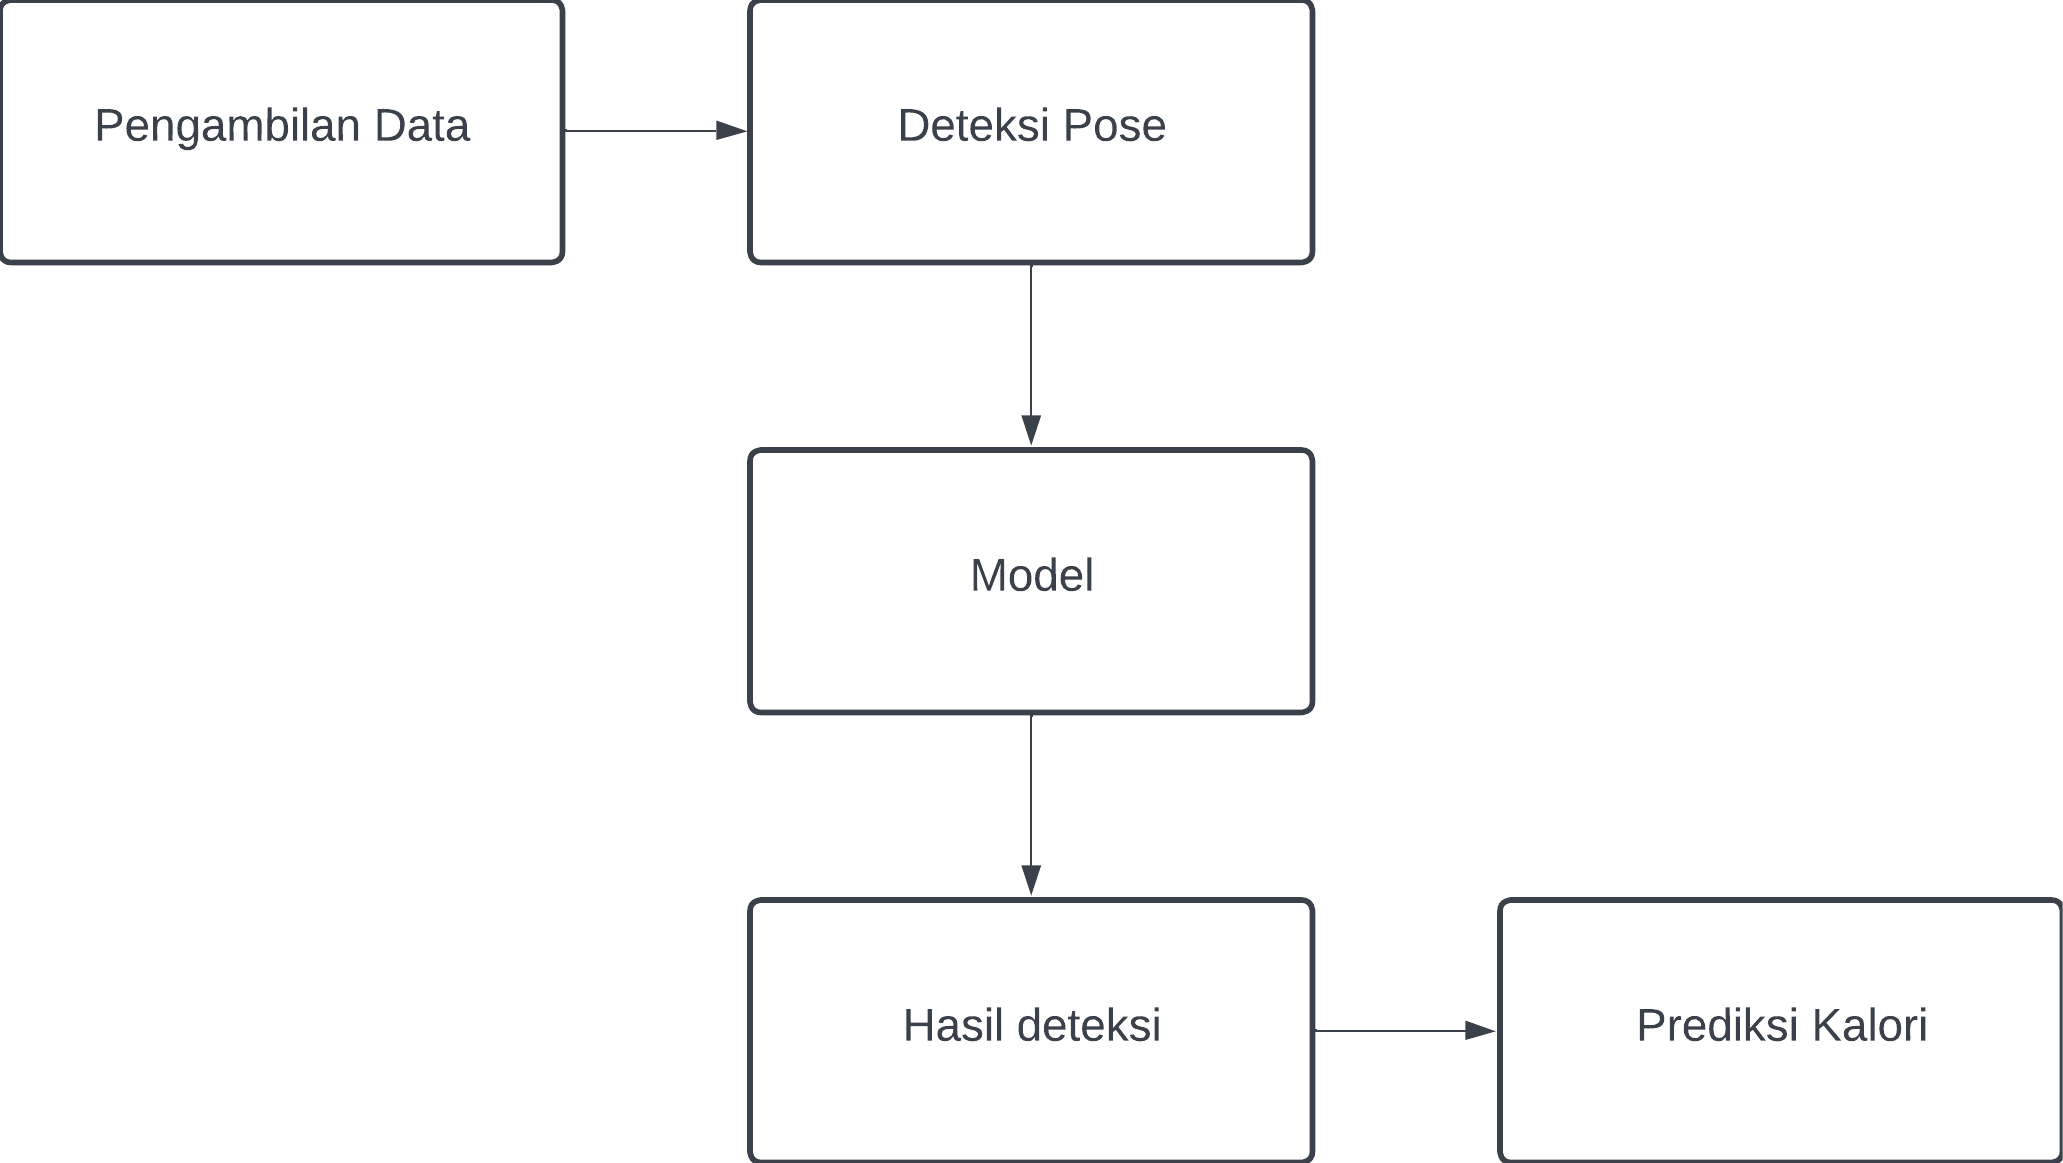
\includegraphics[scale=0.215]{gambar/blok diagram metodologi3.png}
  \caption{Blok Diagram Kerja Sistem}
  \label{fig:BlokDiagram}
\end{figure}

\section{Desain Sistem}
\label{sec:DesainSistem}

Penelitian ini dilaksanakan sesuai \lipsum[1][1-5]

\section{Pengambilan Data}
\label{sec:PengambilanData}

Pada tahap pertama yaitu pengambilan data, data diperoleh menggunakan kamera pada \emph{smartphone} yang akan direkam dan disimpan untuk kemudian akan digunakan pada proses yang dilakukan pada perangkat komputer/laptop atau dapat menggunakan kamera yang dimiliki oleh laptop atau kamera eksternal yang dihubungkan pada laptop ataupun komputer. Proses pengambilan data dilakukan dengan peraga melakukan aktivitas pada treadmill dengan ditampakkan secara jelas pada tampilan kamera. Setelah terdapat peraga dan tampak jelas pada tampilan maka data citra akan dilakukan pada tahap selanjutnya untuk dideteksi dan segmentasi pose seperti pada Gambar \ref{fig:PengambilanData}.

\begin{figure}[H]
  \centering
  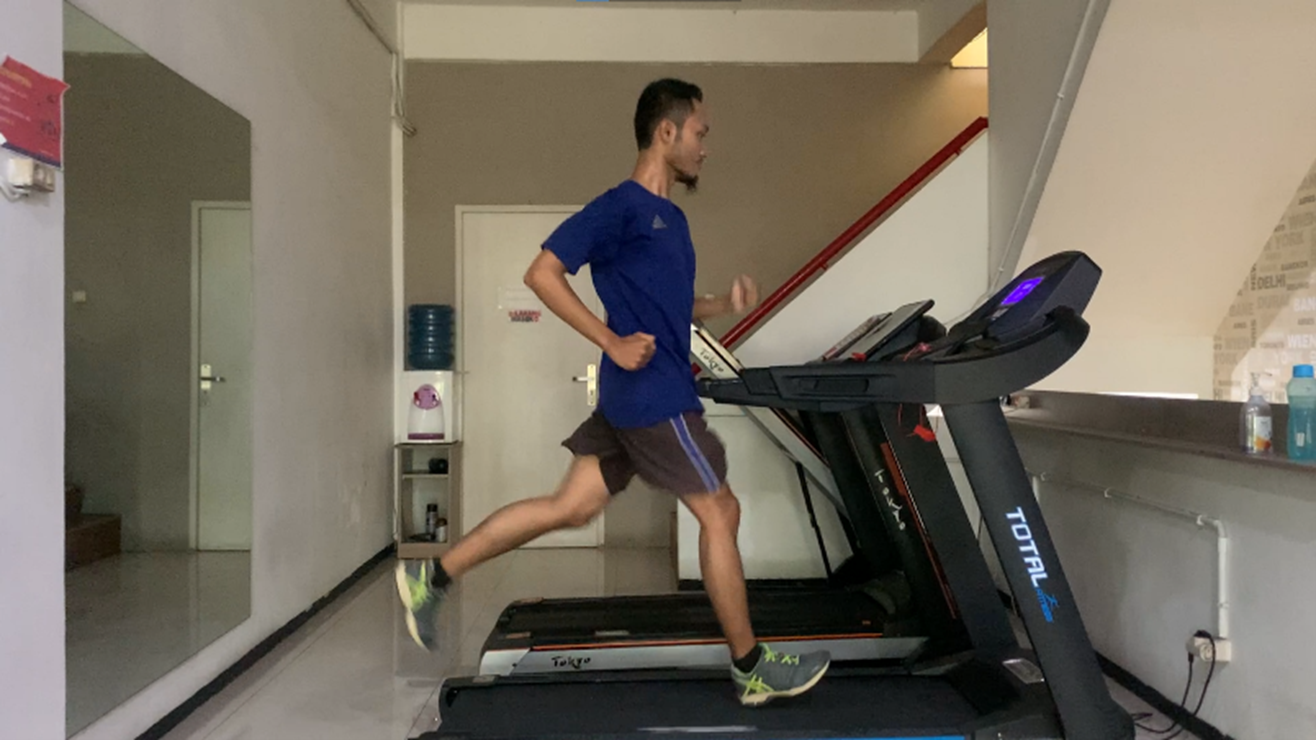
\includegraphics[scale=0.8]{gambar/pengambilan data.png}
  \caption{Proses pengambilan data}
  \label{fig:PengambilanData}
\end{figure}


\section{Deteksi Pose}
\label{sec:DeteksiPose}

Deteksi dari hasil citra untuk dapat mengetahui bentuk postur tubuh manusia menggunakan \emph{Python} dengan \emph{library} OpenCV yaitu MediaPipe. Metode yang digunakan pada MediaPipe menggunakan deteksi pose untuk mendeteksi postur tubuh. Segementasi dilakukan dengan cara peraga melakukan aktivitas jogging pada treadmill dengan menentukan pose melangkah ataupun berlari sesuai dengan olahraga yang akan diteliti. Data yang diproses merupakan data yang telah dilakukan perekaman pada proses pengambilan data dengan menggunakan video yang telah direkam sebelumnya menggunakan alat perekam. Hasil video yang memperlihatkan seseorang dalam keadaan berolahraga pada treadmill melakukan aktivitas berjalan atau berlari akan diproses dalam tahap ini untuk dilakukan deteksi pose. Deteksi pose menggunakan model deteksi yang sudah ada yaitu Mediapipe. Hasil deteksi dari model Mediapipe berupa kerangka yang menyesuaikan bentuk tubuh yang dideteksi dari data video yang dimiliki. Dalam penelitian ini yang berfokuskan pada proses deteksi langkah pada tubuh bagian bawah seperti kaki menyebabkan perlunya pemodelan ulang dan melakukan proses modifikasi pada hasil deteksi model Mediapipe. Dengan begitu proses modifikasi yang dilakukan adalah dengan mengambil kerangka bagian kaki dengan memberikan warna yang berbeda untuk hasil deteksi kaki bagian kiri dan kanan. Proses deteksi pose pada kaki yang dilakukan akan digunakan dalam proses selanjutnya dalam penelitian ini yang digambarkan pada gambar yang terdapat pada Gambar \ref{fig:DeteksiEstimasi}.

\begin{figure}[H]
  \centering
  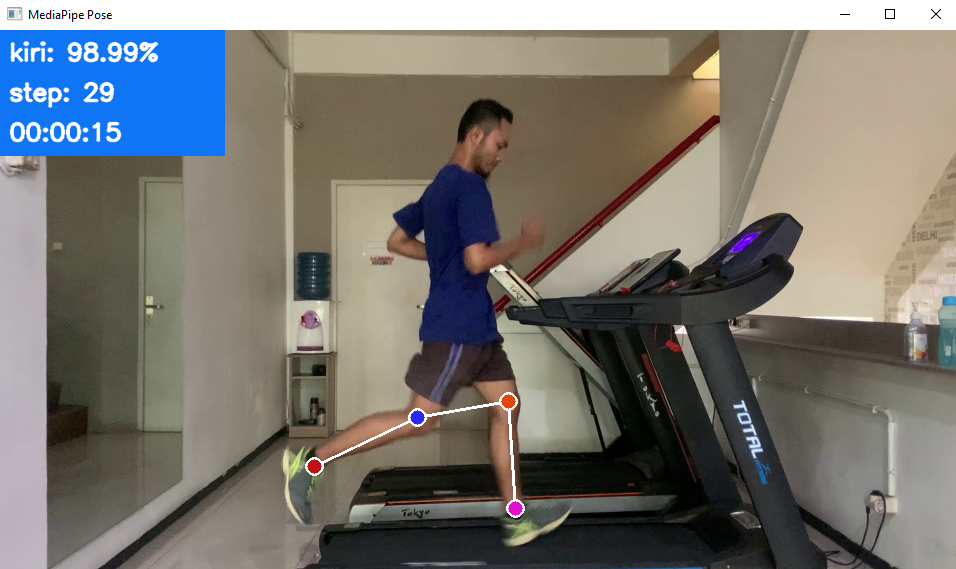
\includegraphics[scale=0.48]{gambar/deteksi pose.png}
  \caption{Deteksi pose dengan MediaPipe}
  \label{fig:DeteksiEstimasi}
\end{figure}

\subsection{\emph{Pre Processing} Data}
\label{subsec:PreProcessingData}

Hasil deteksi pose dengan bentuk kerangka pada kaki sesuai dengan data video dilakukan tahap \emph{Pre Processing}. \emph{Pre Processing} data dilakukan sebagai proses untuk mempersiapkan data dari input yang digunakan untuk kemudian dilakukannya proses pembuatan model dalam tahap \emph{training}. Terdapat beberapa tahapan yang dilakukan pada \emph{pre processing} data untuk kemudian akan didapatkan dataset yang akan dapat digunakan untuk melakukan pembuatan model dengan proses \emph{training}. Setiap data video yang akan digunakan dalam proses ini akan dilakukan ekstrak dari data video menjadi gambar. Data video yang memiliki resolusi sebesar 1920 x 1080 dengan 25 FPS akan diubah dan diekstrak menjadi satuan gambar untuk digunakan sebagai dataset melalui proses \emph{pre processing} data. Dengan resolusi data demikian akan menghasilkan 25 gambar atau \emph{frame} setiap satu detik dari video tersebut. Hasil ekstrak gambar dalam \emph{Pre Processing} data ini akan kemudian dilanjutkan dalam proses untuk membuat dataset untuk kemudian digunakan dalam proses \emph{training} menjadi model.

\subsection{Augmentasi Data}
\label{subsec:AugmentasiData}

Pada proses deteksi pose didapat hasil deteksi pada data video berupa kerangka pada kaki yang menyesuaikan bentuk tubuh yang sedang ditampilkan. Setelah dapat dideteksi dengan baik menggunakan model Mediapipe dan dimodifikasi untuk dapat terfokus pada bagian kaki, dilakukan proses augmentasi data. Augmentasi data dilakukan sebagai proses untuk mengubah atau memodifikasi gambar agar dapat dengan mudah diproses dalam tahap \emph{training}. Proses ini juga akan dapat membantu dalam meningkatkan akurasi dari model yang akan digunakan nanti karena data telah diproses dan dimodifikasi agar memiliki data-data tambahan yang akan berguna dalam tahap \emph{training}. 

Data dari proses deteksi pose akan dilakukan proses pemindahan hasil deteksi kerangka ke dalam gambar baru dengan penyesuaian yang akan digeneralisasikan terhadap semua data yang didapat. Proses dimulai dengan menentukan posisi kerangka dari data video asli untuk kemudian akan dipindahkan ke gambar baru. Dalam melakukan menentukan posisi kerangka dilakukan dengan deteksi menggunakan bingkai yang menyesuaikan posisi keseluruhan kerangka yang dapat dilihat pada Gambar \ref{fig:PreProcessing1}. Setelah bingkai menyesuaikan posisi kerangka maka akan dipindahkan pada gambar dengan latar belakang hitam yang berisikan hanya kerangka dari hasil deteksi sesuai dengan bingkai. Proses melakukan pemindahan hasil deteksi ke dalam gambar dengan latar belakang hitam dapat ditunjukan pada gambar Gambar \ref{fig:PreProcessing2}. Kemudian gambar akan dilakukan generalisasi terhadap ukuran yang berisikan hanya hasil deteksi sesuai bingkai untuk mempermudah dalam proses selanjutnya dengan membuat ukuran gambar seragam dalam bentuk persegi.

\begin{figure}[H]
  \centering
  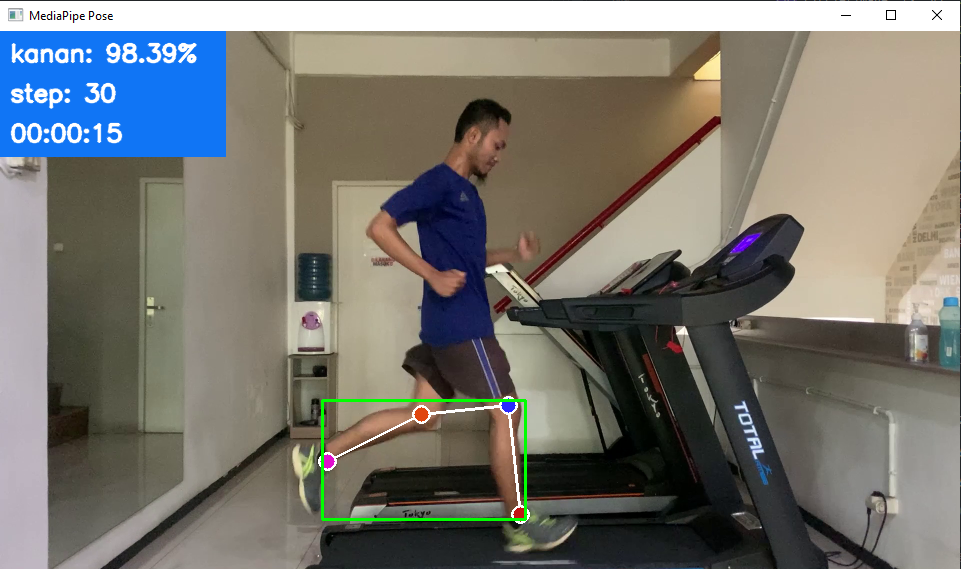
\includegraphics[scale=0.48]{gambar/deteksi pose2.png}
  \caption{\emph{Pre Processing} hasil deteksi pose dengan bingkai}
  \label{fig:PreProcessing1}
\end{figure}

\begin{figure}[H]
  \centering
  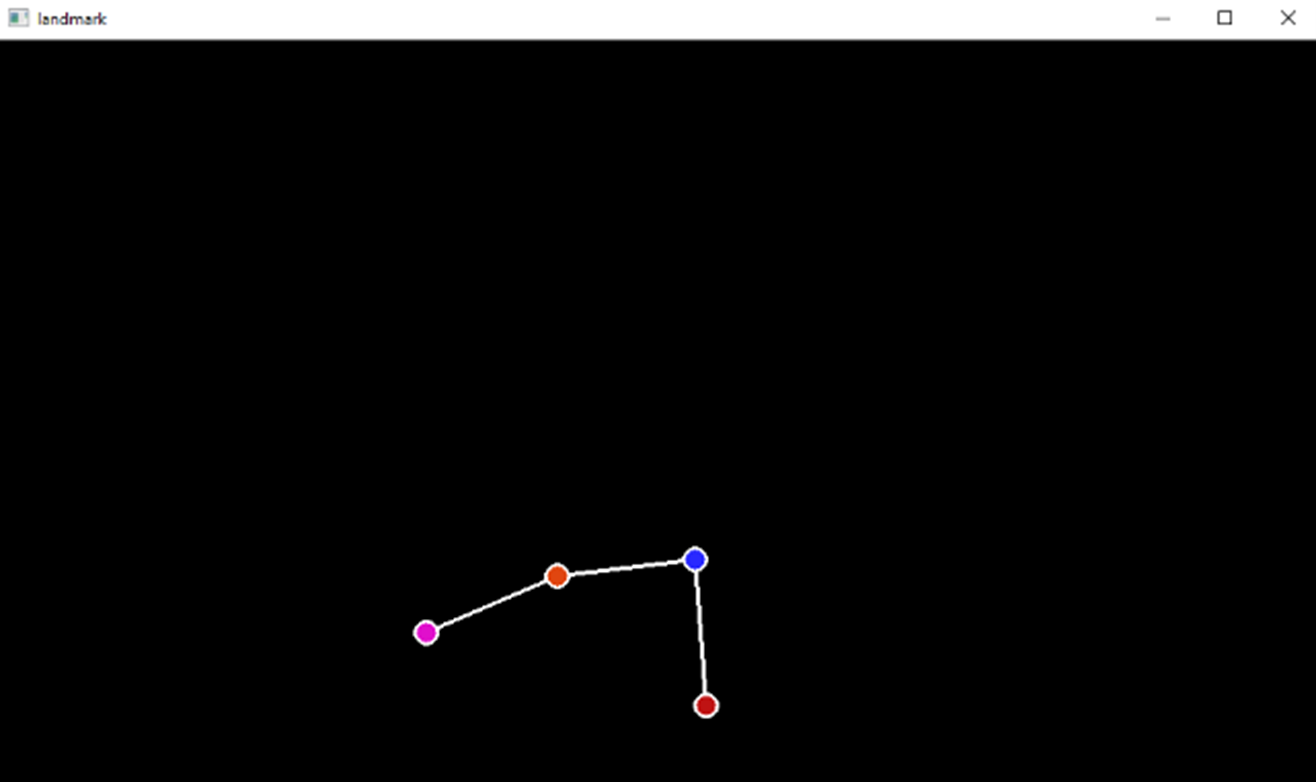
\includegraphics[scale=0.8]{gambar/deteksi pose3.png}
  \caption{\emph{Pre Processing} hasil deteksi pose pada latar belakang hitam}
  \label{fig:PreProcessing2}
\end{figure}

\subsection{Pelabelan Objek}
\label{subsec:PelabelanObjek}

Hasil dari proses augmentasi data dengan melakukan pemindahan hasil deteksi ke dalam gambar baru yang telah disesuaikan akan diproses menjadi sebuah dataset. Pelabelan objek diperlukan untuk dapat memberikan informasi nama kelas dari objek yang akan dideteksi pada penelitian ini. Proses pada pelabelan objek ini dilakukan setelah didapatkan proses dalam \emph{pre processing} dengan mengekstrak data video menjadi gambar dan dilakukan proses augmentasi dari setiap data gambar yang didapat. Kemudian dari hasil augmentasi dengan memiliki hasil gambar kerangka berdasarkan hasil deteksi dikelompokkan pada kategori atau kelas yang berbeda. Pada penelitian ini proses deteksi yang diinginkan adalah dapat menentukan proses aktivitas melangkah atau berlari dengan mengetahui kaki kanan atau kiri yang sedang berada di depan. Dengan begitu kelas yang dimiliki pada dataset yang akan dibuat dengan terdapat dua label atau kelas yaitu kanan dan kiri. Hasil ekstraksi dan augmentasi yang dilakukan berdasarkan kelas yang diinginkan dapat dilihat untuk kelas kanan pada Gambar \ref{fig:KelasKanan} dan untuk kelas kiri pada Gambar \ref{fig:KelasKiri}.

\begin{figure}[H]
  \centering
  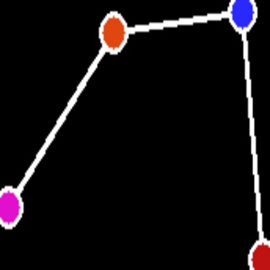
\includegraphics[scale=0.8]{gambar/dataset kanan.png}
  \caption{Hasil \emph{pre processing} untuk kelas kanan}
  \label{fig:KelasKanan}
\end{figure}

\begin{figure}[H]
  \centering
  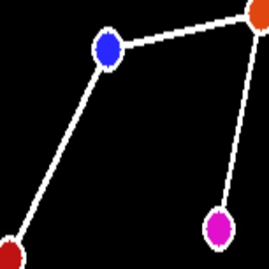
\includegraphics[scale=0.8]{gambar/dataset kiri.png}
  \caption{Hasil \emph{pre processing} untuk kelas kiri}
  \label{fig:KelasKiri}
\end{figure}


\subsection{Dataset}
\label{subsec:Dataset}

Dataset yang digunakan pada penelitian ini berdasarkan hasil dari data video yang dimiliki dengan mengambil sampel pada proses pengambilan data. Kemudian dilakukan proses \emph{pre processing} dengan melakukan ekstraksi gambar, augmentasi data, dan pelabelan objek yang akan disimpan keseluruhan data yang dimiliki berdasarkan kelas untuk menjadi dataset yang akan digunakan pada penelitian ini. Dataset yang telah dimiliki pada penelitian ini berupa data gambar berisikan bentuk kerangka dari hasil deteksi dengan model Mediapipe yang telah dimodifikasi dan digeneralisasi untuk ukuran gambar. Hasil dari dataset yang akan digunakan untuk dataset kelas kanan ditunjukkan pada Gambar \ref{fig:DatasetKanan} dan untuk dataset kelas kiri ditunjukkan pada Gambar \ref{fig:DatasetKiri}.

\begin{figure}[H]
  \centering
  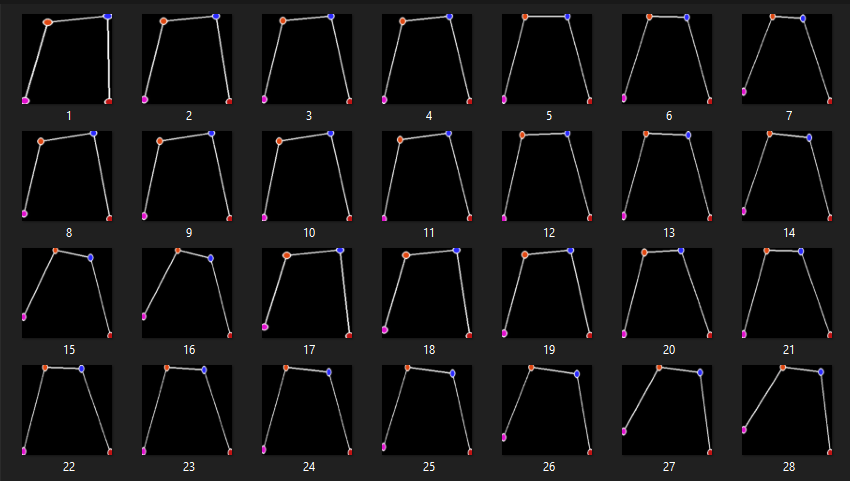
\includegraphics[scale=0.5]{gambar/folder dataset kanan.png}
  \caption{Dataset untuk kelas Kanan}
  \label{fig:DatasetKanan}
\end{figure}

\begin{figure}[H]
  \centering
  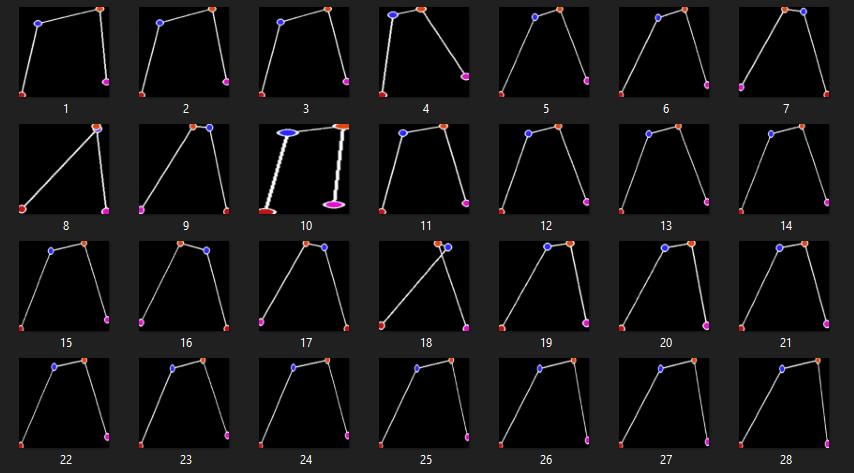
\includegraphics[scale=0.5]{gambar/folder dataset kiri.png}
  \caption{Dataset untuk kelas Kiri}
  \label{fig:DatasetKiri}
\end{figure}


\section{Model}
\label{sec:Klasifikasi}

Dataset yang telah dimiliki maka kemudian dilakukan \emph{training} untuk memperoleh model deteksi. Model deteksi dari dataset akan digunakan untuk melatih model dari sebuah algoritma pada \emph{Machine Learning}. Dalam melakukan klasifikasi menggunakan \emph{Convolutional Neural Networks} (CNN). Proses \emph{training} ini bertujuan agar nantinya komputasi yang dilakukan dalam proses deteksi akan dapat diolah berdasarkan akuisisi data citra yang ingin dideteksi menjadi bentuk atau pola pemahaman yang diinginkan. Hasil \emph{training} akan didapatkan model yang digunakan untuk melakukan klasifikasi atas dataset yang dimiliki yaitu terdapat dua kelas atau label untuk dapat diklasifikasikan menjadi kaki kanan dan kiri. Klasifikasi dalam menentukan aktivitas yang digunakan pada penelitian ini adalah dapat mengetahu langkah dari seseorang yang berjalan atau berlari. Hasil klasifikasi dari model yang telah dibuat untuk menentukan hasil deteksi untuk kelas kanan ditunjukkan pada Gambar \ref{fig:KlasifikasiKanan} dan hasil deteksi untuk kelas kiri ditunjukkan pada Gambar \ref{fig:KlasifikasiKiri}.

\begin{figure}[H]
  \centering
  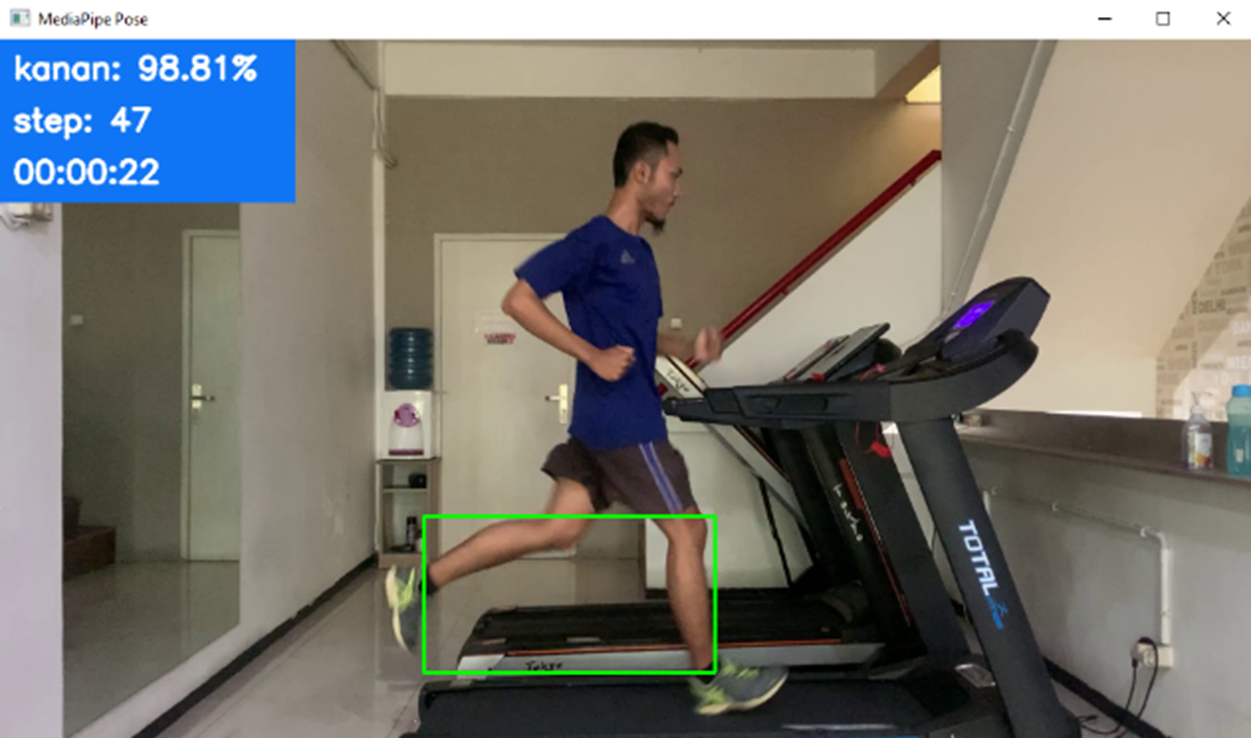
\includegraphics[scale=0.8]{gambar/klasifikasi kanan.png}
  \caption{Klasifikasi untuk kelas kanan}
  \label{fig:KlasifikasiKanan}
\end{figure}

\begin{figure}[H]
  \centering
  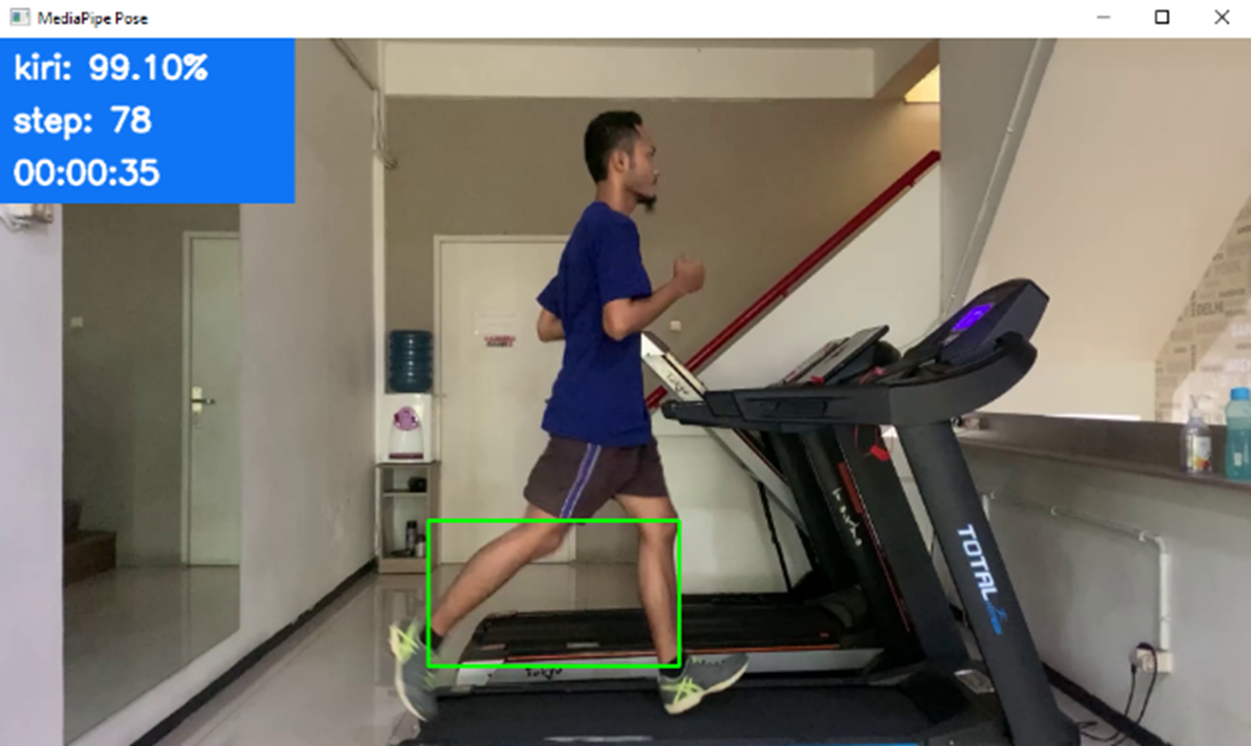
\includegraphics[scale=0.8]{gambar/klasifikasi kiri.png}
  \caption{Klasifikasi untuk kelas kiri}
  \label{fig:KlasifikasiKiri}
\end{figure}


\section{Hasil Deteksi}
\label{sec:HasilDeteksi}

Bentuk hasil klasifikasi yang dibuat adalah mendeteksi pose aktivitas dengan dapat menghitung langkah dan waktu yang ditempuh. Nilai langkah dan waktu yang ditempuh akan digunakan dalam perhitungan selanjutnya. Banyaknya jumlah langkah yang didapat saat hasil deteksi digunakan sebagai nilai variable pertama yang akan digunakan dalam penentuan perhitungan kalori. Langkah dideteksi dan dihitung seberapa banyak langkah yang dilakukan saat proses deteksi. Waktu tempuh saat proses deteksi merupakan nilai variabel kedua yang akan digunakan dalam penentuan perhitungan kalori. Waktu tempuh dimulai saat dideteksi pertama kali nilai langkah yang ditemukan hingga saat akhir langkah tidak ada penambahan kembali yang menandakan proses deteksi telah selesai. Hasil deteksi akan ditampilkan seiring dengan proses deteksi yang dilakukan pada data citra seperti pada Gambar \ref{fig:HasilDeteksi} dan pada akhir proses deteksi akan menampilkan hasil akumulasi akhir dari hasil deteksi terhadap deteksi langkah dan waktu tempuh. Selain itu juga terdapat tampilan hasil perhitungan dan prediksi yang diharapkan dalam penelitian ini. Hasil tampilan untuk hasil deteksi di akhir sebagai akumulasi deteksi ditunjukkan pada Gambar \ref{fig:HasilDeteksi2}.

\begin{figure}[H]
  \centering
  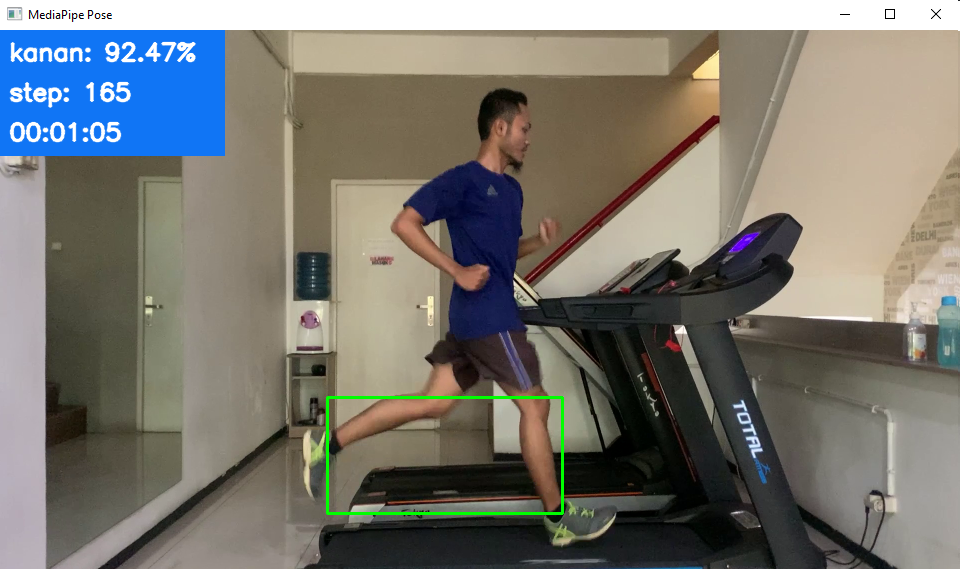
\includegraphics[scale=0.48]{gambar/hasil deteksi.png}
  \caption{Tampilan hasil deteksi saat proses deteksi}
  \label{fig:HasilDeteksi}
\end{figure}

\begin{figure}[H]
  \centering
  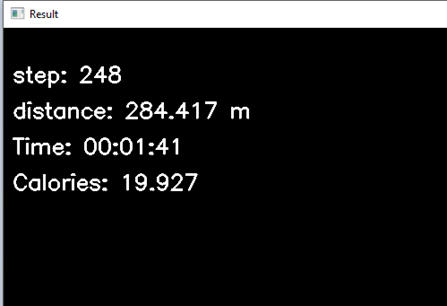
\includegraphics[scale=0.8]{gambar/hasil deteksi2.png}
  \caption{Tampilan akumulasi hasil deteksi}
  \label{fig:HasilDeteksi2}
\end{figure}

\subsection{Hasil Deteksi Langkah}
\label{subsec:HasilLangkah}

Banyaknya jumlah langkah yang didapat saat hasil deteksi digunakan sebagai nilai variable pertama yang akan digunakan dalam penentuan perhitungan kalori. Langkah dideteksi dan dihitung seberapa banyak langkah yang dilakukan saat proses deteksi. Nilai banyaknya jumlah langkah akan disimpan dan akan digunakan pada saat proses perhitungan kalori setelah proses deteksi telah selesai dilakukan.

\subsection{Hasil Waktu Tempuh}
\label{subsec:HasilWaktu}

Waktu tempuh saat proses deteksi merupakan nilai variabel kedua yang akan digunakan dalam penentuan perhitungan kalori. Waktu tempuh dimulai saat dideteksi pertama kali nilai langkah yang ditemukan hingga saat akhir langkah tidak ada penambahan kembali yang menandakan proses deteksi telah selesai. Nilai waktu akan dibutuhkan dalam satuan waktu menit untuk proses perhitungan kalori.

\section{Prediksi Kalori}
\label{sec:PrediksiKalori}

Prediksi kalori dilakukn dengan dua metode, yaitu menggunakan metode regresi linear dan menggunakan perhitungan rumus EC (Exercise Calories) berdasarkan satuan ukuran MET (Metabolic Equivalent). Kedua metode prediksi ini digunakan sebagai pembanding dalam melakukan analisa terhadap hasil yang didapatkan dari metode prediksi menggunakan metode regresi linear dengan perhitungan rumus. Data yang digunakanan dalam proses prediksi kalori diambil berdasarkan hasil klasifikasi dan hasil deteksi yang telah dilakukan sebelumnya. Hasil deteksi berupa banyaknya langkah dan waktu tempuh digunakan untuk proses prediksi kalori baik dengan metode regresi linear maupun metode perhitungan rumus.

\subsection{Regresi Linear}
\label{subsec:PrediksiRegresi}

Regresi merupakan suatu teknik analisis untuk mengidentifikasi relasi antar dua variabel atau lebih. Model regresi linear dilakukan dengan cara membuat dataset terlebih dahulu yang diatur sesuai dengan variabel-variabel yang dibutuhkan pada penelitian ini. Terdapat variabel independen dan variabel dependen sebagai bentuk model dataset yang akan digunakan pada regresi linear yang digunakan. Variabel independen yang digunakan pada dataset ini adalah waktu tempuh dan jarak tempuh. Sedangkan untuk variabel dependen yang digunakan adalah jumlah kalori yang terbakar.

Dalam membuat model regresi linear, perlu dilakukan training dan pencarian dataset terlebih dahulu menggunakan alat bantu treadmill yang memiliki perhitungan jumlah kalori yang terbakar dengan menvariasikan sebanyak-banyaknya variabel yang akan digunakan pada model regresi linear. Setelah melakukan percobaan dan pencarian dataset maka akan didapatkan dataset untuk model regresi linear. Dengan didapatkannya model regresi linear, maka saat melakukan akuisisi data citra untuk diprediksi jumlah pembakaran kalori dengan menghasilkan hasil deteksi yang akan diregresikan dengan model regresi yang telah dimiliki dapat dilakukan prediksi jumlah pembakaaran kalori dari data citra tersebut.

\subsection{Perhitungan Rumus}
\label{subsec:PrediksiPerhitungan}

Perhitungan kalori dilakukan dengan mengacu pada nilai satuan ukuran MET (Metabolic Equivalent). Satuan MET akan mendapat pengukuran untuk konsumsi oksigen dan pembakaran kalori. Nilai dari satuan MET dapat didefinisikan pada Persamaan 1.

\begin{equation}
  \label{eq:SatuanMET}
  1 \mathbf{MET} = 3,5 ml O_2  / KG / min
\end{equation}

Berdasarkan nilai satuan ukuran MET, didapatkan suatu persamaan untuk menghitung pembakaran kalori yang didefiniskan pada Persamaan 2.

\begin{equation}
  \label{eq:RumusKalori}
  \mathbf{Cal} = \frac{MET x 3,5 x BB}{200} calories / min
\end{equation}

Pada persamaan pembakaran kalori yang akan digunakan untuk melakukan perhitungan pembakaran kalori dari aktivitas yang dilakukan dibutuhkan beberapa nilai variabel untuk mendapatkah hasil total pembakaran kalori, yaitu nilai MET, nilai berat badan (BB), dan nilai waktu tempuh dalam menit.

Setiap aktivitas memiliki nilai MET yang berbeda-beda dan telah ditentukan oleh peneliti yang telah merangkum banyak aktivitas untuk ditentukan berapa nilai MET yang dihasilkan. Pada aktivitas olahraga yang difokuskan saat ini adalah jogging pada treadmill juga memiliki perbedaan nilai MET yang dipengaruhi oleh kecepatan jogging. Kecepatan aktivitas jogging dapat diketahui dengan nilai hasil deteksi berupa banyak langkah dan waktu tempuh untuk menentukan kecepatan dengan menggunakan Persamaan 3.

\begin{equation}
  \label{eq:RumusKecepatan}
  \mathbf{Kecepatan} = \frac{Jarak}{Waktu}
\end{equation}

Untuk nilai jarak dilakukan dengan melakukan model regresi polinomial dari panjang langkah dari hasil kali kecepatan dan waktu yang dibagi dengan banyak langkah sesuai dataset yang diperoleh dari pengumpulan data pada treadmill. Model regresi digunakan untuk menentukan panjang jarak yang akan digunakan saat melakukan akuisisi data citra untuk dilakukan prediksi dengan menghasilkan data banyak langkah dan waktu tempuh. Kemudian banyak langkah akan dikalikan dengan hasil regresi untuk mentukan panjang langkah dan hasil pengalian tersebut dibagi dengan waktu tempuh untuk menemukan kecepatan. Dengan diperolehnya kecepatan maka dapat menentukan MET dengan membuat model regresi MET berdasarkan data yang telah dilakukan peneliti dan dapat dilanjutkan untuk mengetahui kalori dengan menggunakan rumus pada Persamaan 1.
